\newpage
\section{Scenario 1 - Angle Range}\label{sec:scenario1}
The first scenario describes the movement of the antennas when the UA flies far away from the GS between two predefined positions (Figure \ref{fig:s1_map}). The distance between the aircraft and the GS can be represented by a parabola, as is described in Figure \ref{fig:s1_los}. In the beginning, the distance between both devices is around 48km and, while the UA is flying, the distance becomes smaller, achieving a minimum value. After this minimum, the distance between the devices increases until the UA reach the final position.

Based on Figures \ref{fig:s1_pd_gs_alone} and \ref{fig:s1_pd_ua_alone}, it is possible to observe that the azimuth and elevation angles of the UA and the GS often have different behaviours during the whole movement. 

\begin{figure}[H]
	\centering
	\subfigure[UAS Map Positioning]{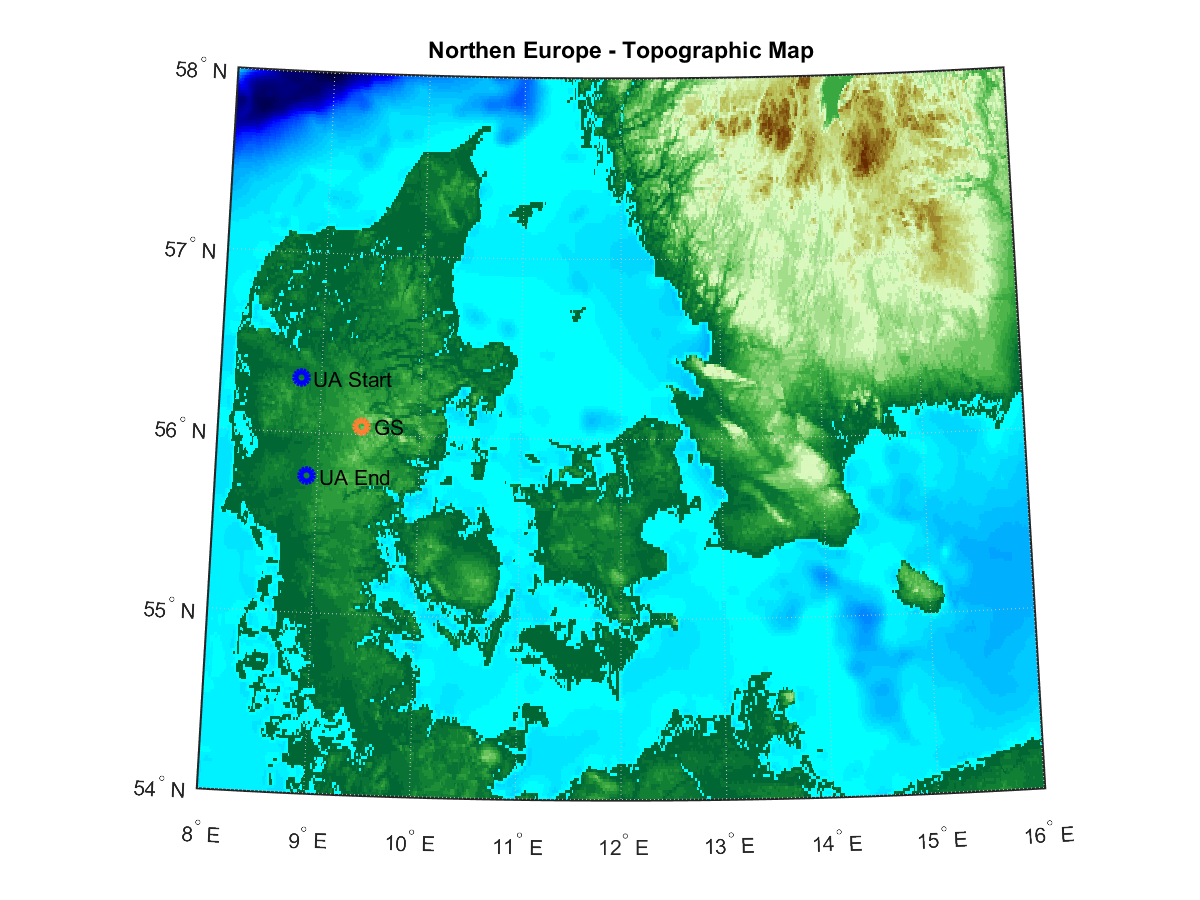
\includegraphics[scale=0.42]{figures/s1_map.png}}
	\\
	\subfigure[UAS Map Zoom]{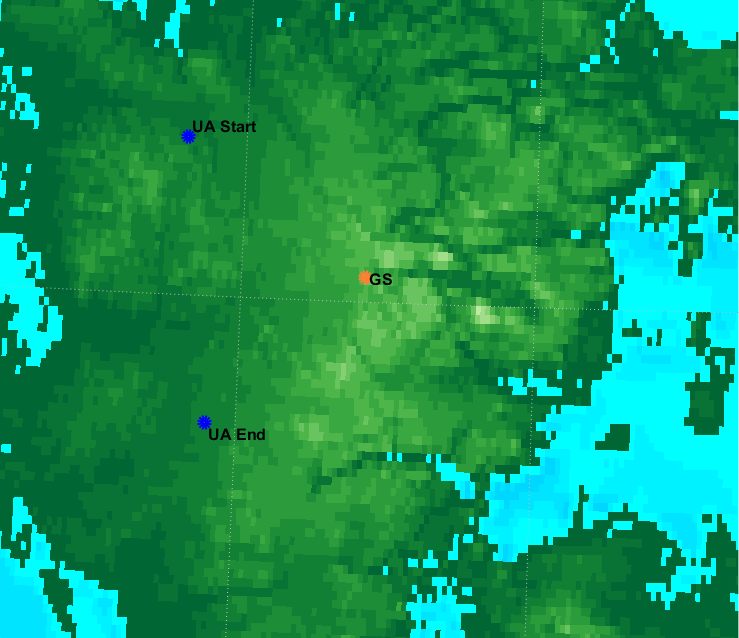
\includegraphics[scale=0.33]{figures/s1_zoom.png}}
	\caption{Angle Range Scenario}
	\label{fig:s1_map}
\end{figure}

\begin{figure}[H]
	\centering
	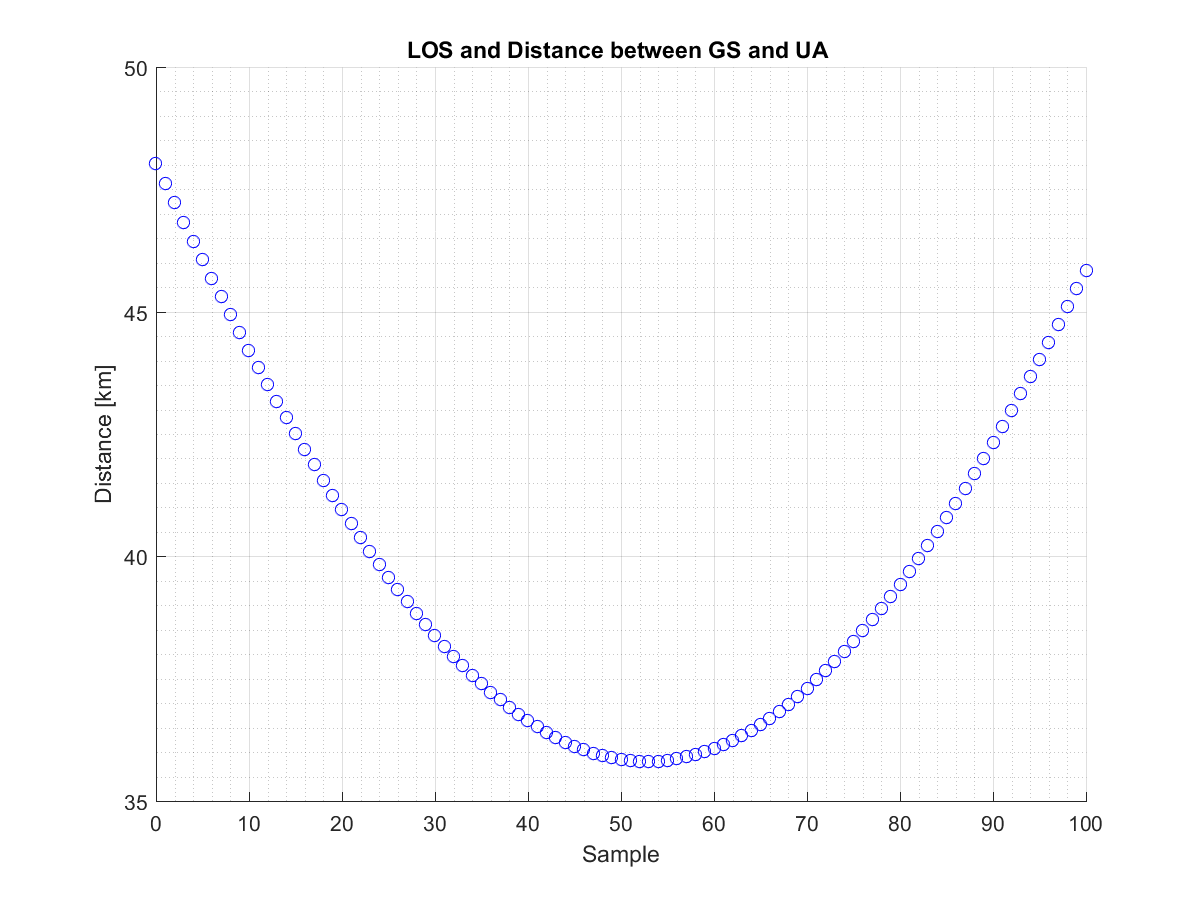
\includegraphics[scale=0.7]{figures/s1_los.png}
	\caption{LOS and Distance}
	\label{fig:s1_los}
\end{figure}

\subsection*{GS Tracking Angles}\label{GroundStation_scenario1}
As expected, the absolute value of the $\theta_{OPTIMAL}$ increases (Figure \ref{fig:s1_pd_gs_alone}) until it reaches 180$^{\circ}$  and, then, it starts increasing from -180$^{\circ}$ until the end. The initial $\theta_{OPTIMAL}$ is around 140$^{\circ}$ due to the system of coordinates applied where the Local NED frame coincides with the body frame. This assumption was taken into account because the position of the GS is static.

In the beginning, the azimuth angle is positive and growing due to the fact that the UA is flying on the left side of the GS (lower longitude) to thee south (decreasing latitude). However, there is a jump when $\theta$ reaches 180$^{\circ}$ in the first graph of Figure \ref{fig:s1_pd_gs_alone}. This happens due to the used convention which limits the range from -180$^{\circ}$ to 180$^{\circ}$. Nonetheless, there is a continuous rotation, which means that when the antenna achieves 180$^{\circ}$, it will continue rotate in the same direction starting from -180$^{\circ}$. Thus, after the jump, the azimuth angle will continue to increase from -180$^{\circ}$ until -136$^{\circ}$.

On the other hand, the optimal elevation angle, $\phi_{OPTIMAL}$, has always a small amplitude because of the important distance between the UA and the GS of the second graph of Figure \ref{fig:s1_pd_gs_alone}. Since the previous distance is always bigger than 36km, a considerable optimal $\phi$ is not required to point at the UA. 

Despite of the small amplitude, $\phi_{OPTIMAL}$ has a maximum value (approximately 0.06$^{\circ}$) which corresponds to the minimum distance between the UA and the GS (closest point). Therefore, when the UA is closer, the GS’s antenna needs to increase the angle in order to be able to continue pointing at the antenna of the aircraft.

\begin{figure}[H]
	\centering
	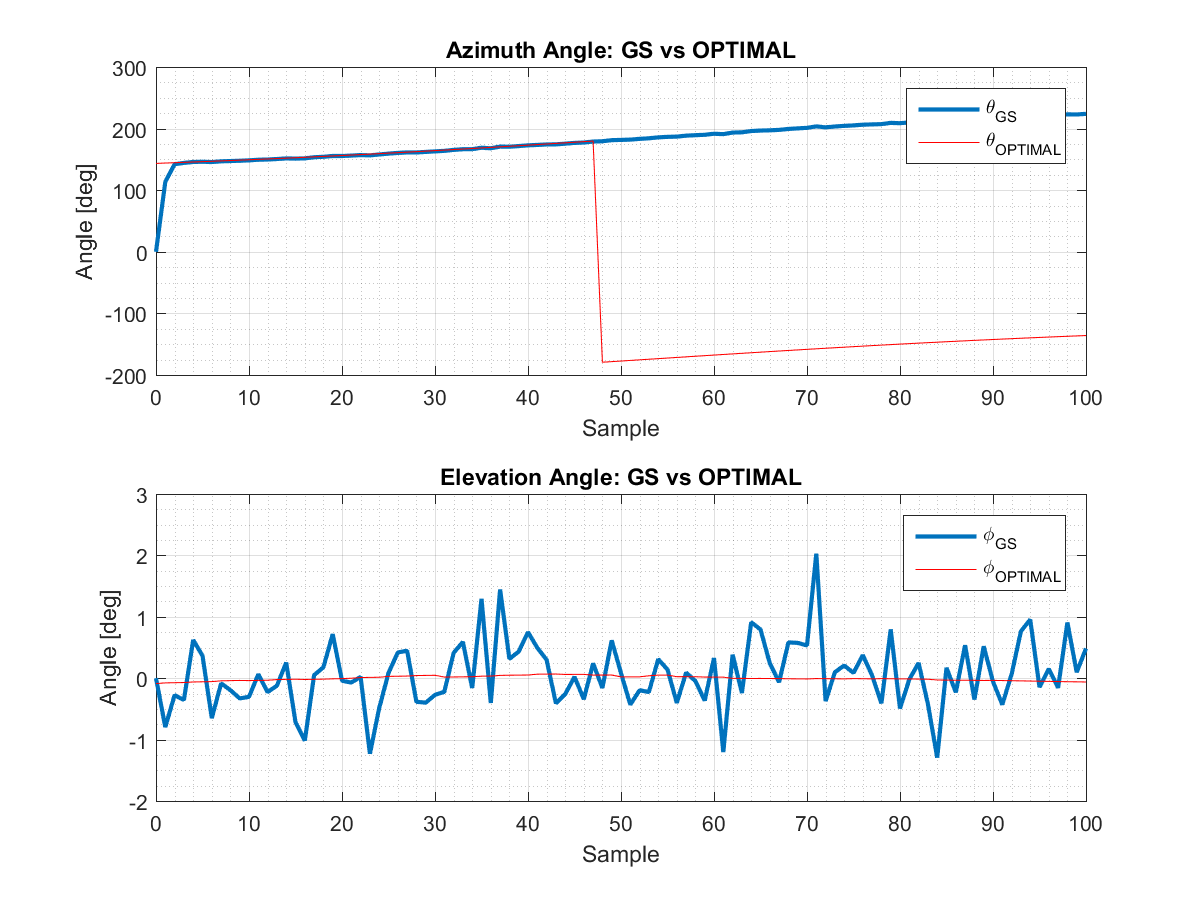
\includegraphics[scale=0.75]{figures/s1_pd_gs.png}
	\caption{Behaviour of the azimuth and elevation angles of the antenna in the GS during the movement of the UA}
	\label{fig:s1_pd_gs_alone}
\end{figure}

The previous explanation describes generally how the angles of the antennas change during the flight of the UA, taking into account the azimuth and elevation angles. However, there are some details related to the response that depend on the type of P-I-D controllers that are applied in the system. Figure \ref{fig:s1_gs} represents the behaviour of P, PI, PD and PID controllers for the given scenario.

Based on the simulations of the controllers described on Section \ref{sec:controller} and on the azimuths plots of Figure \ref{fig:s1_gs}, it is possible to verify that the PI and PID controllers have an overshoot, while the P and PD follow directly the desired response. The integral term in the PI and PID controllers is the one responsible for the overshoots due to the accumulation of the error during the whole process. In practice, the antenna starts rotating in order to achieve the desired angle. However, it achieves the requested angle with a high velocity that do not allow the antenna to stop on time. Thus, the antenna continues rotating until it stops and inverses the way of the movement. Then, rotating in the opposite direction, the antenna achieves the desired angle and follows the optimal response. On the other hand, PID controller is faster than the PI controller because of the damping effect of the derivative term.

In this project, P and PD controllers are not affected by the overshoot and, furthermore, the \emph{PD controller is the fastest controller (lowest rise time)} due to its derivative component.

\begin{figure}[H]
	\centering
	\subfigure[P Controller]{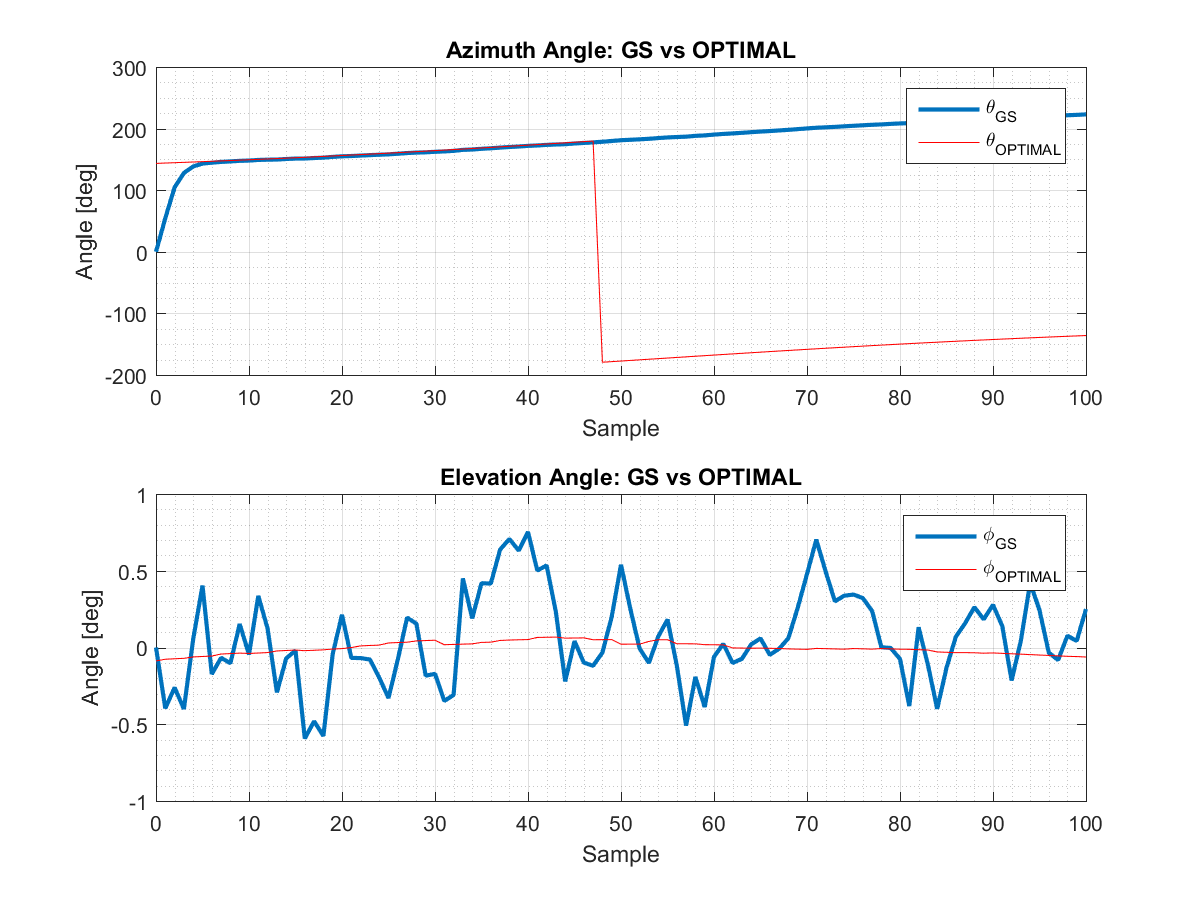
\includegraphics[scale=0.45,angle=-90]{figures/s1_p_gs.png}}
	\hfill
	\subfigure[PI Controller]{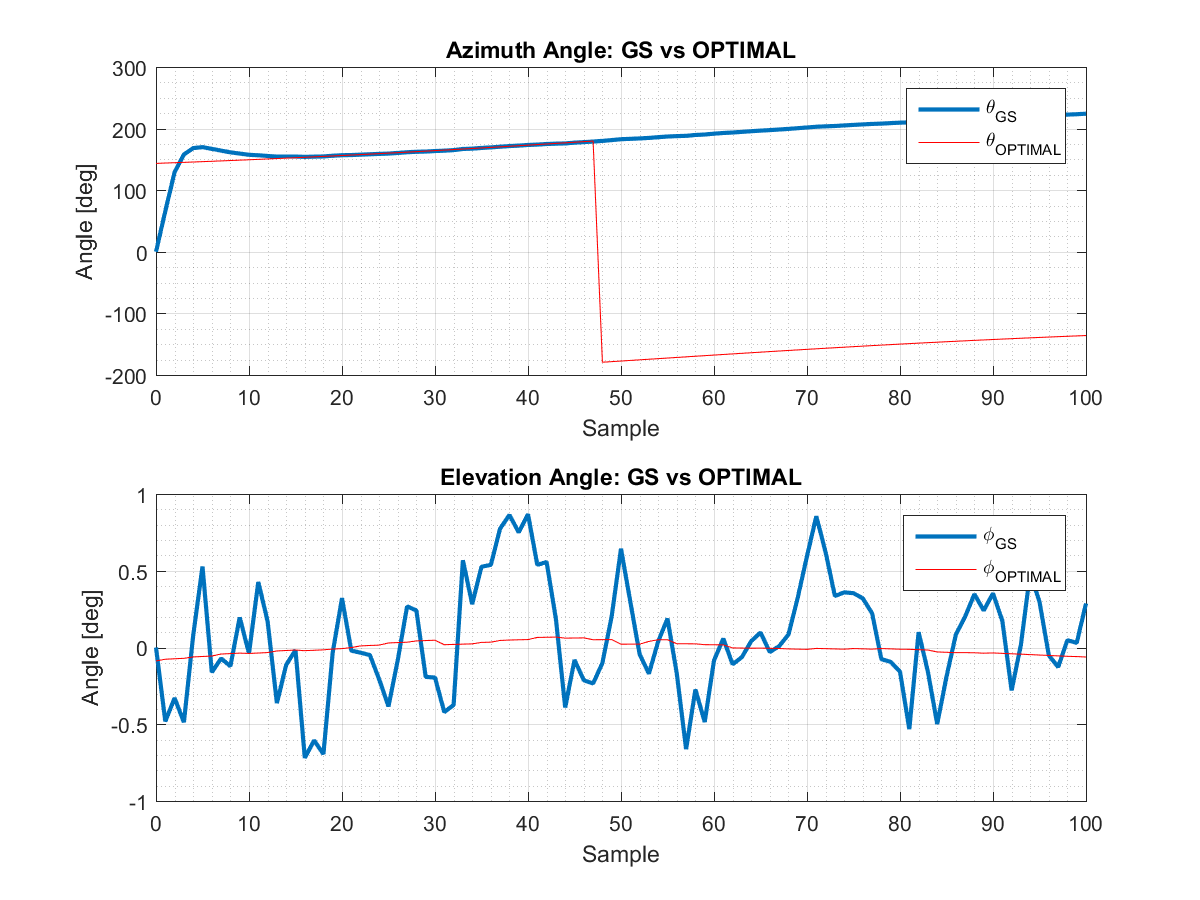
\includegraphics[scale=0.45,angle=-90]{figures/s1_pi_gs.png}}
	\\
	\subfigure[PD Controller]{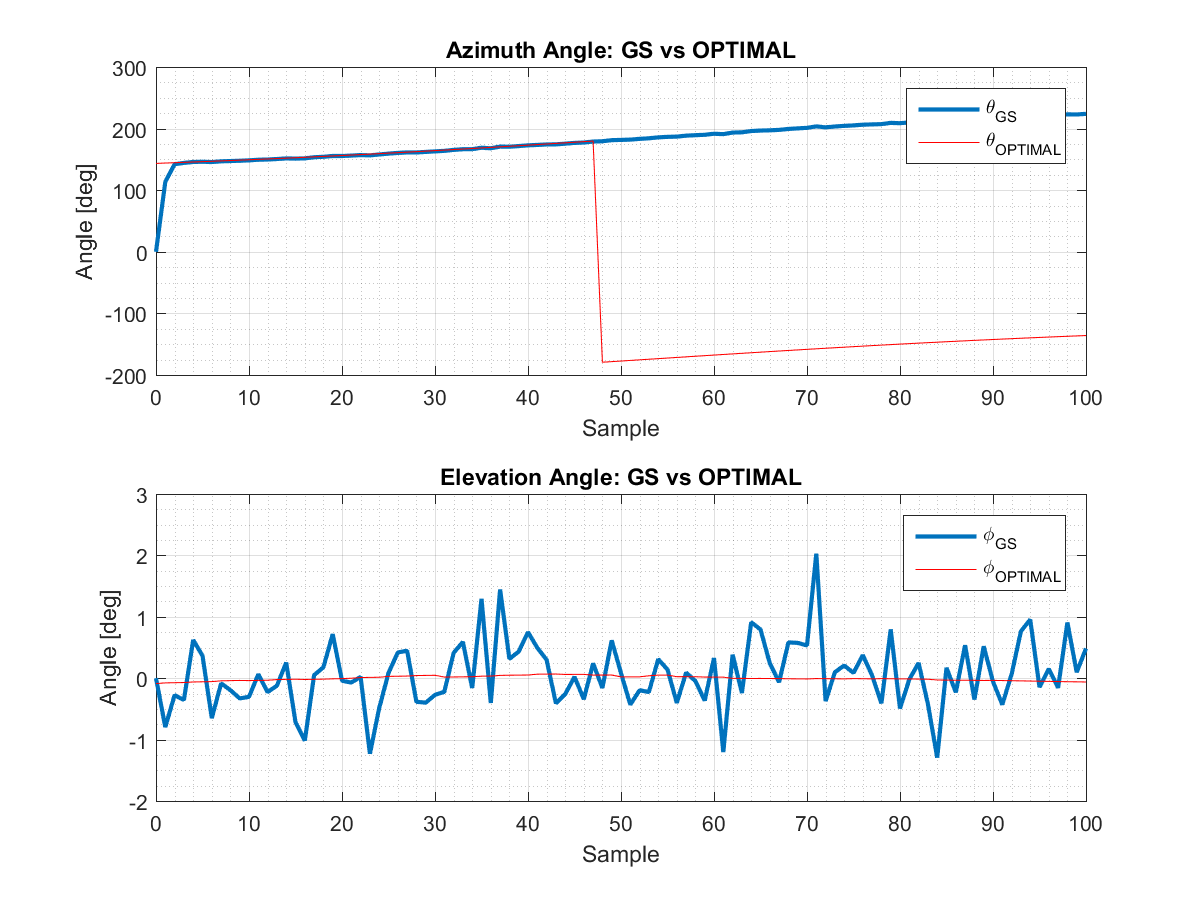
\includegraphics[scale=0.45,angle=-90]{figures/s1_pd_gs.png}}
	\hfill
	\subfigure[PID Controller]{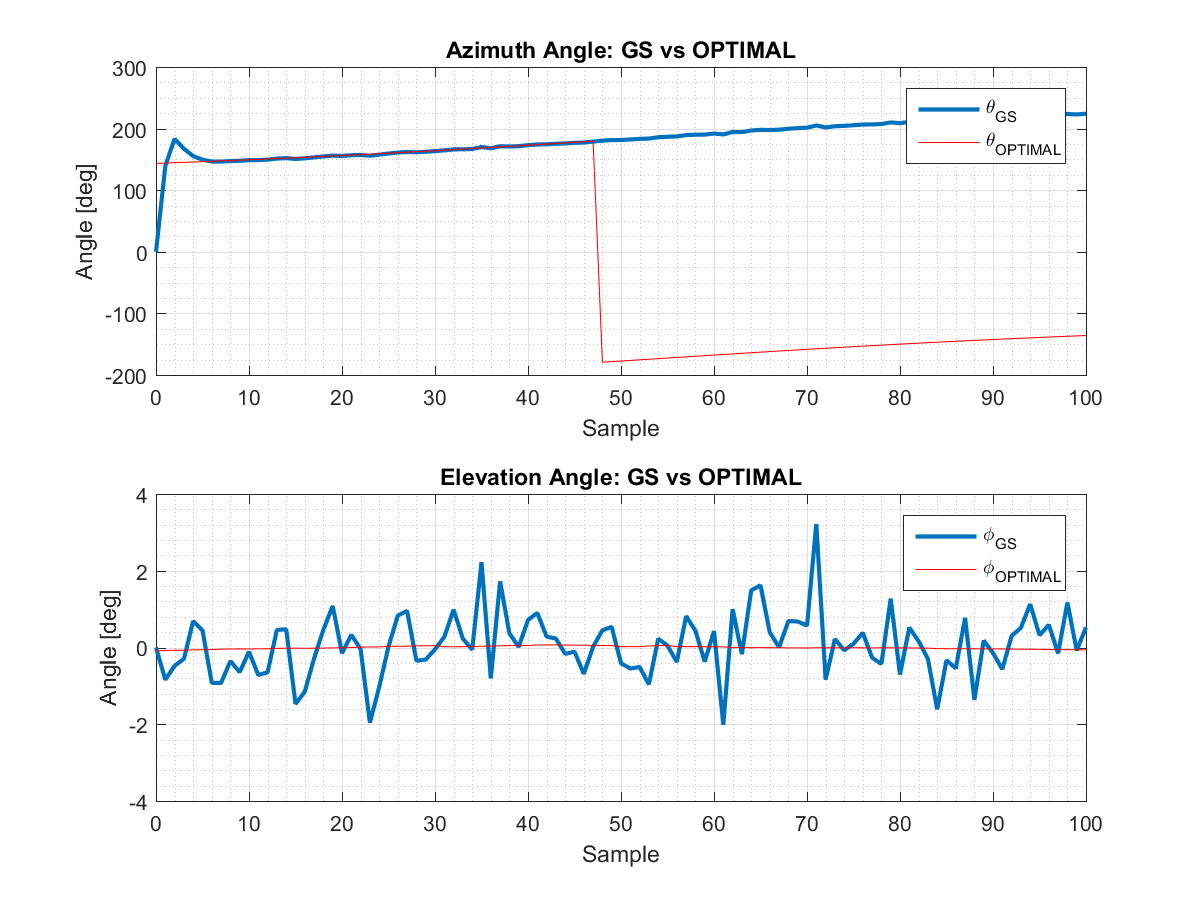
\includegraphics[scale=0.45,angle=-90]{figures/s1_pid_gs.png}}
	\caption{Ground Station Controllers}
	\label{fig:s1_gs}
\end{figure}

\subsection*{UA Tracking Angles}
Figure \ref{fig:s1_pd_ua_alone} shows the elevation and azimuth angles of the UA during the whole movement. Based on the fact that the Local NED frame does not coincide with the body frame, it is possible to understand the behaviour of the angle of the antenna. Since the GS is in the right side of the UA (bigger longitude) and the UA is flying towards south (decreasing latitude), the antenna angle will be positive during the whole flight.
The initial $\theta_{OPTIMAL}$ starts around 50$^{\circ}$ and, as was mentioned before, it increases until around 130$^{\circ}$.

The optimal elevation angle, $\phi$, of the UA has almost the same behaviour as the one of the GS. This means that the angle has a small value because there is considerable distance between the UA and the GS in the second graph of Figure \ref{fig:s1_pd_ua_alone}. Although, in this case, the $\phi_{OPTIMAL}$ has a minimum value instead of a maximum one. This happens because the altitude of the UA is bigger than the one of the GS which demands the antenna to point down.


\begin{figure}[H]
	\centering
	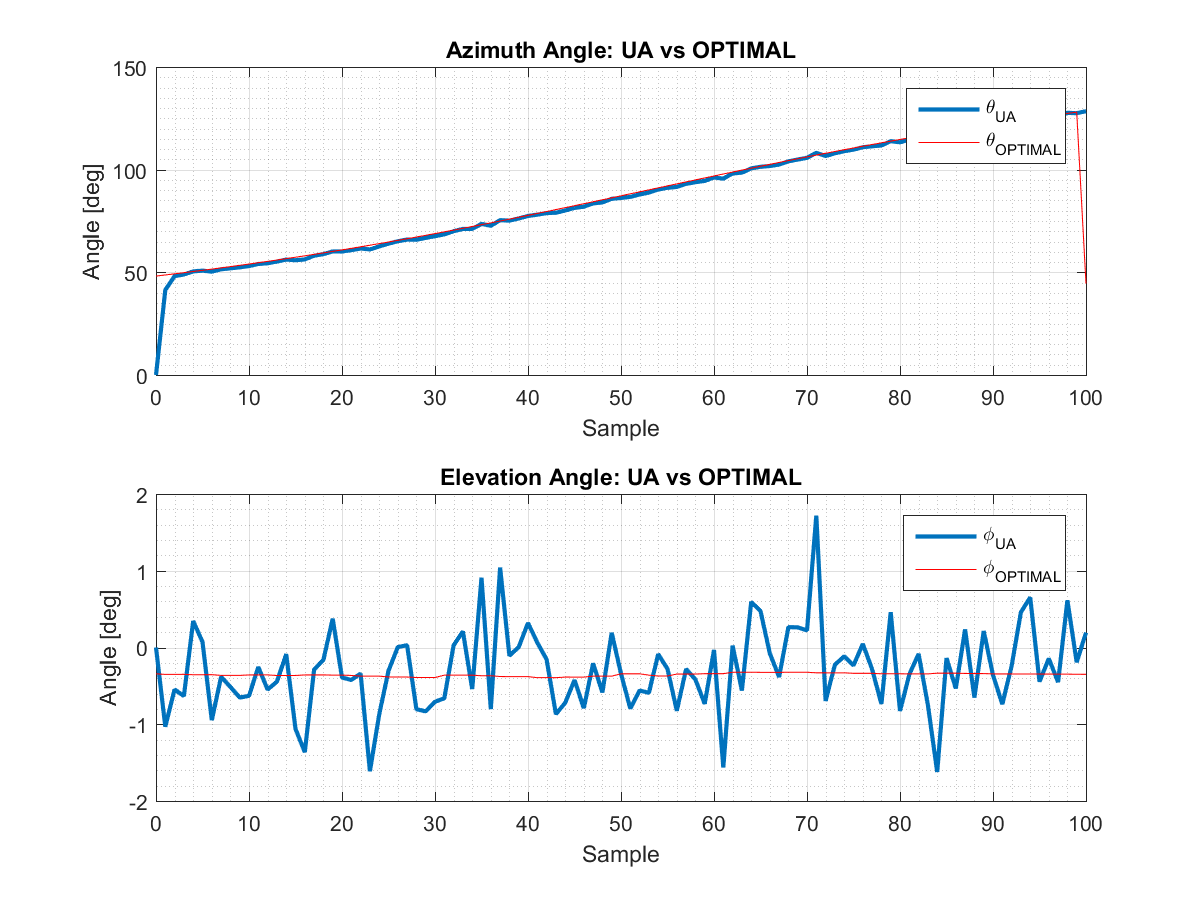
\includegraphics[scale=0.75]{figures/s1_pd_ua.png}
	\caption{Behaviour of the azimuth and elevation angles of the antenna in the UA during its own flight}
	\label{fig:s1_pd_ua_alone}
\end{figure}

The controllers used in this section are the same ones that were used to test the behaviour of the antenna in the GS. This means that the performance will be similar to the ones illustrated in Figure \ref{fig:s1_gs}.

Thus, based on the graphs of the azimuth angle of Figure \ref{fig:s1_ua}, it is observable that the PI and PID controllers have an overshoot when the system is trying to achieve the desired position. Moreover, the response of the system with the P and PD controllers immediately achieve the desired angle, without any overshoot.

\begin{figure}[H]
	\centering
	\subfigure[P Controller]{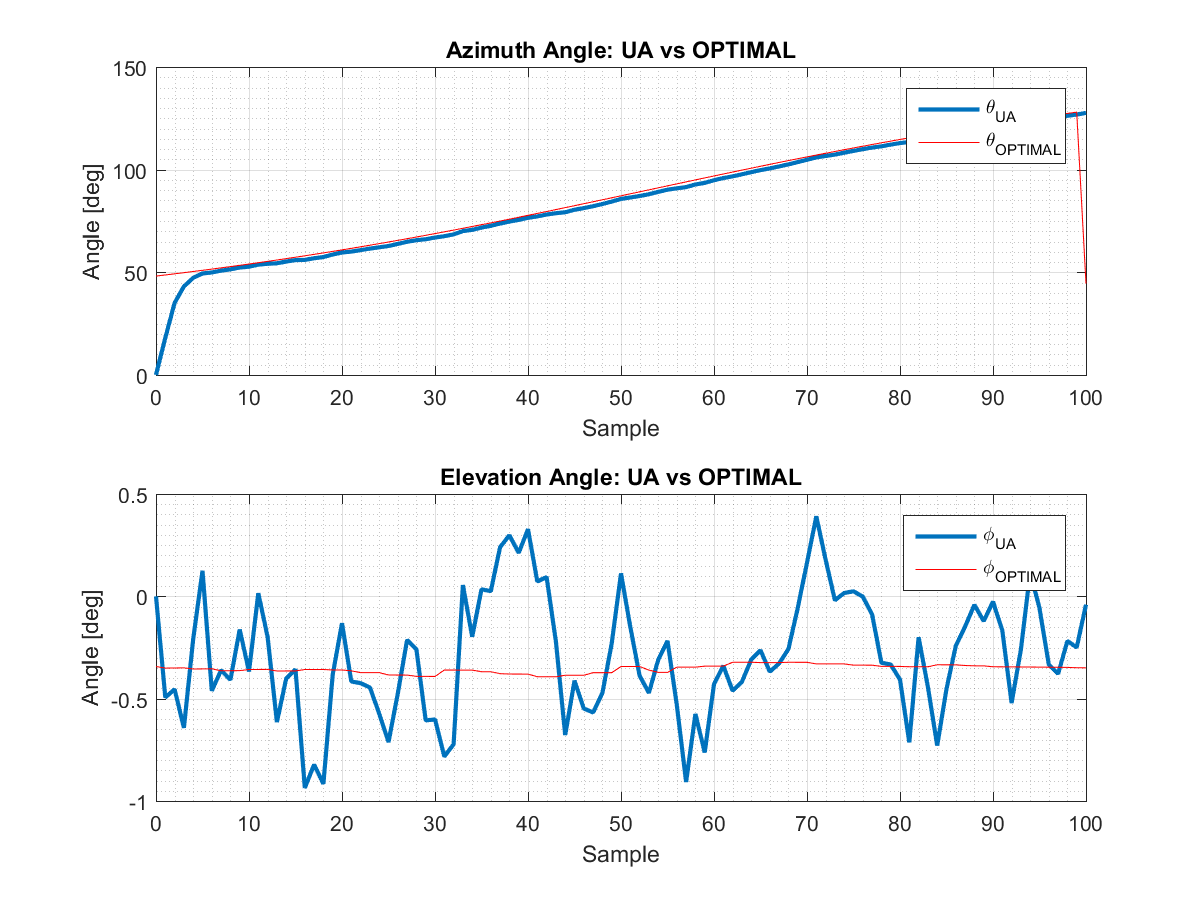
\includegraphics[scale=0.45,angle=-90]{figures/s1_p_ua.png}}
	\subfigure[PI Controller]{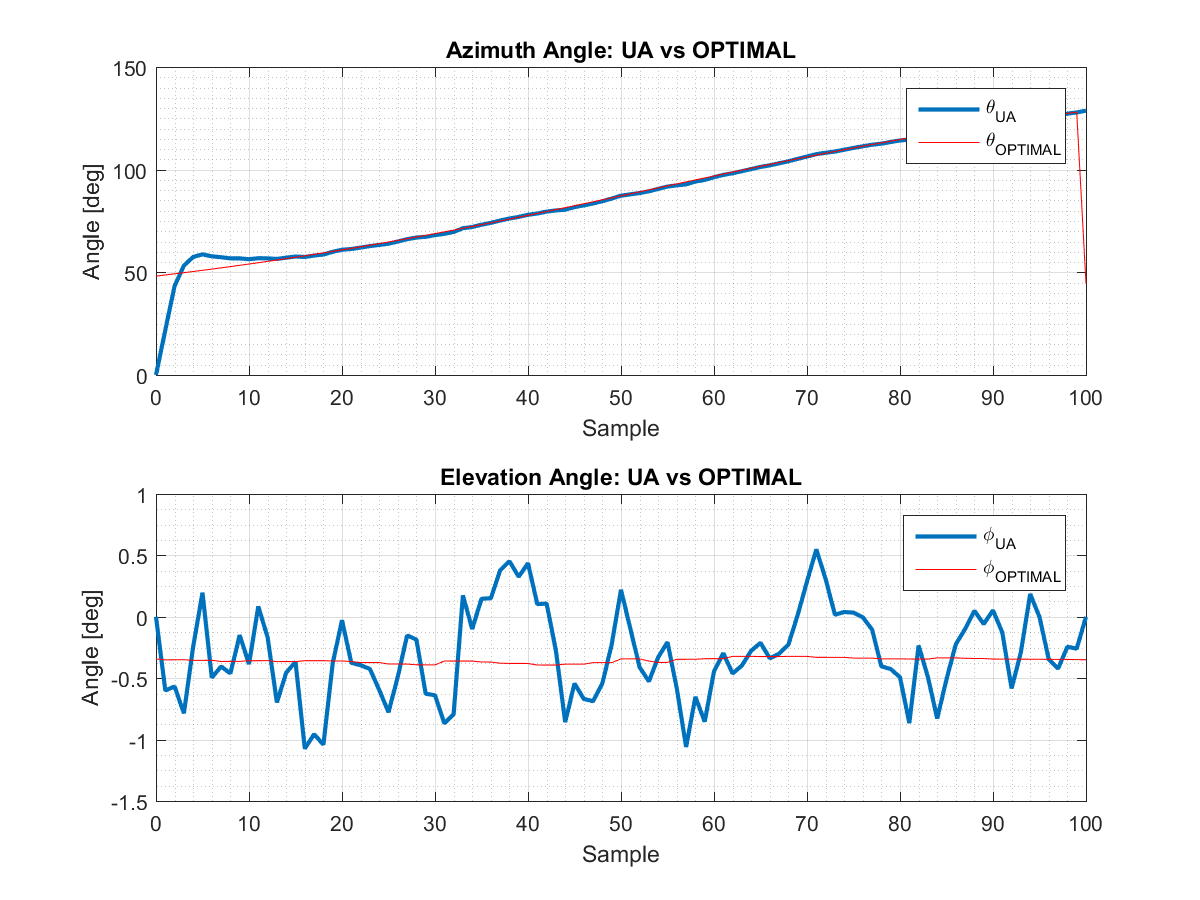
\includegraphics[scale=0.45,angle=-90]{figures/s1_pi_ua.png}}
	\\
	\subfigure[PD Controller]{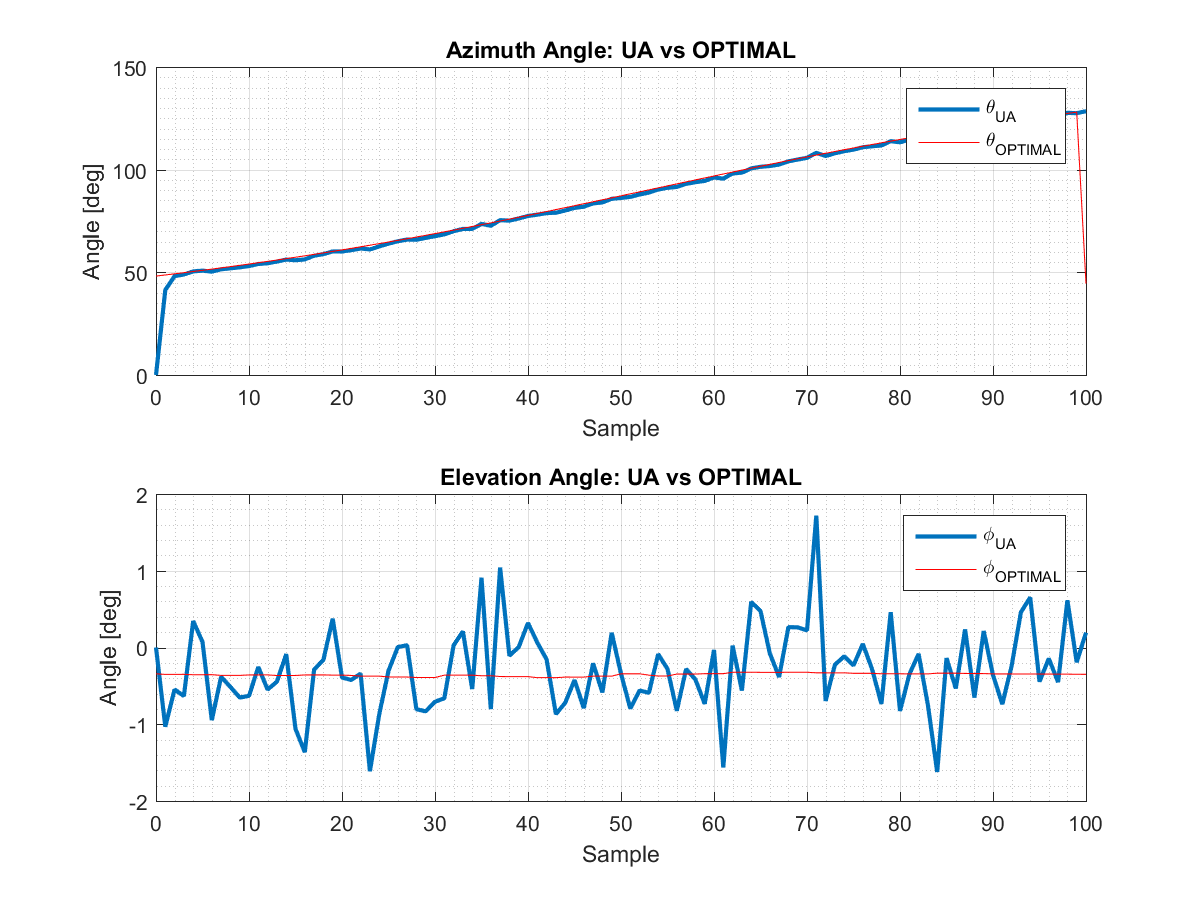
\includegraphics[scale=0.45,angle=-90]{figures/s1_pd_ua.png}}
	\hfill
	\subfigure[PID Controller]{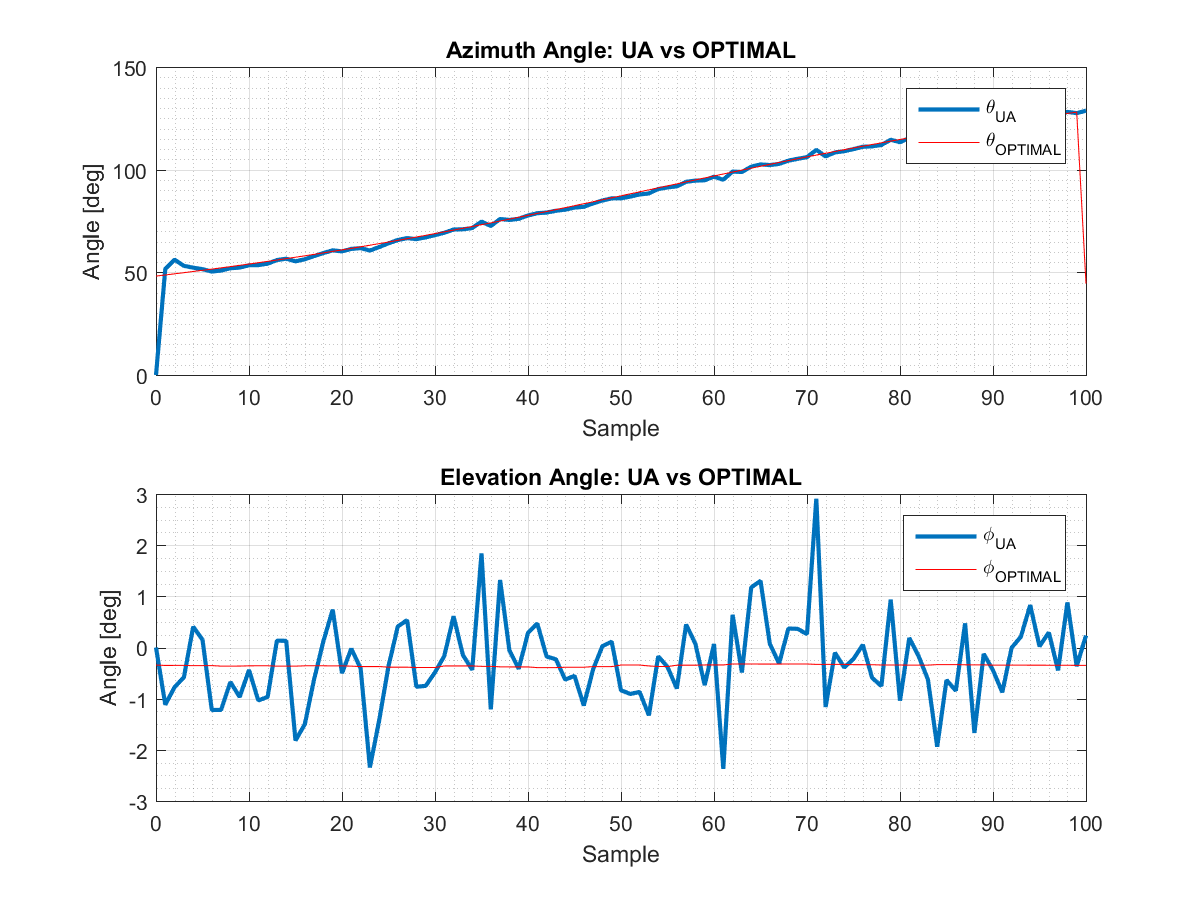
\includegraphics[scale=0.45,angle=-90]{figures/s1_pid_ua.png}}
	\caption{Unmanned Aircraft Controllers}
	\label{fig:s1_ua}
\end{figure}

\subsection*{Signal Power}
In general, the power at the receiver described in Figure \ref{fig:s1_power} has almost the same behaviour in all of the different controllers. In every case, the signal power in the beginning is weak (-100dBm) because the antennas are not pointing at each other. After 10 samples, the antenna of the GS and the antenna of the UA are pointing at each other and the power received in all cases is the same (antennas in the GS and in the UA are the same in all cases). Since they are pointing at each other, in an ideal situation, the maximum power only depends on the kind of antennas used.

When the UA is at the closest point to the GS, the power in the receiver has a peak at the time sample of 54. This happens because the distance between the antennas is small which reduces the path losses.

On the other hand, all plots have a different reaction between the moment when the antennas start moving until the one when they achieve the desired position. This happens because there are details that depend on the type of controller that is used to manage the movement of the antennas. 

As was described in the previous sections, the P and PD controllers do not have any overshoot. This fact allows both controllers to achieve the maximum power faster than the PI and PID. These ones are affected by the overshoot, which means that they achieve the maximum power but, since they continue the rotation, the connection is weakened. Thus, the power received decreases sharply until the antenna change the direction of rotation.


\begin{figure}[H]
	\hfill
	\subfigure[P]{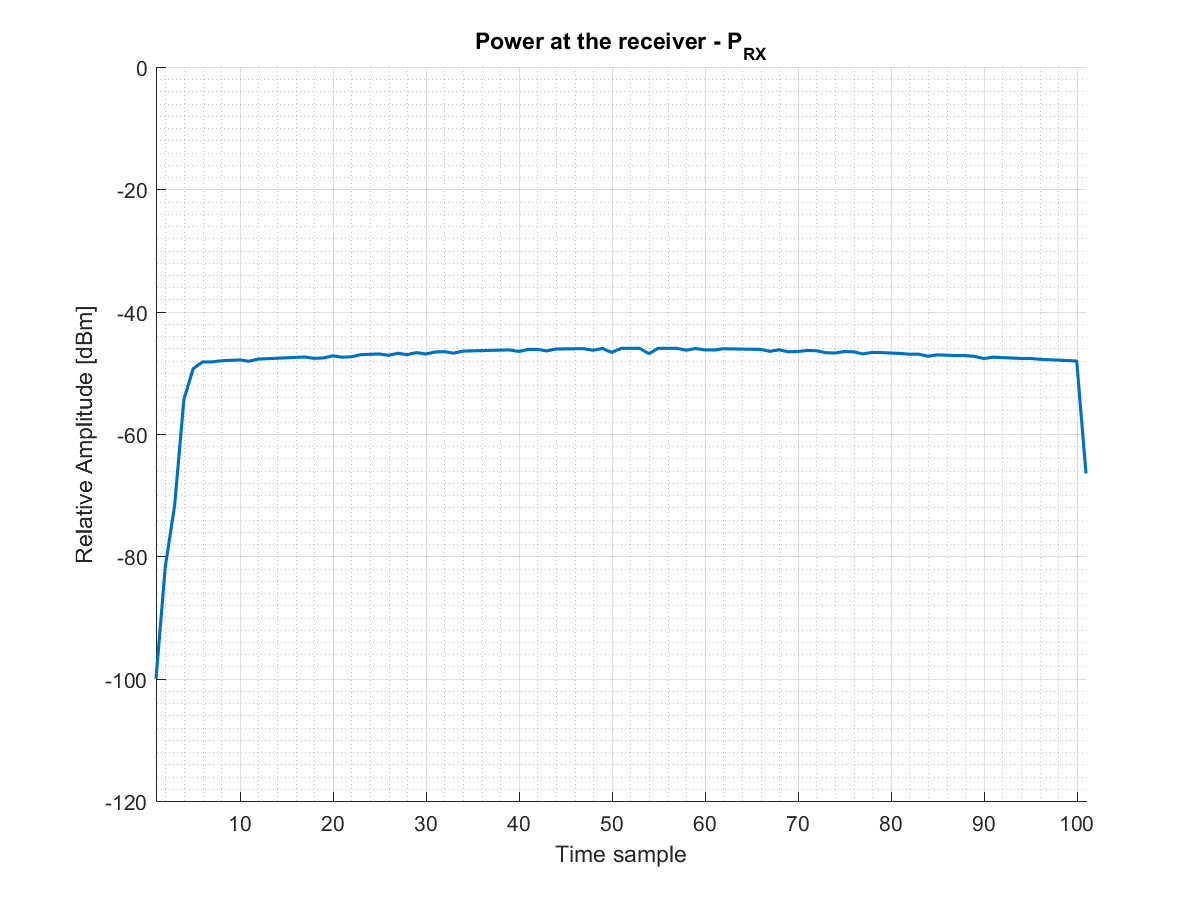
\includegraphics[scale=0.45,angle=-90]{figures/s1_p_power.png}}
	\hfill
	\subfigure[PI]{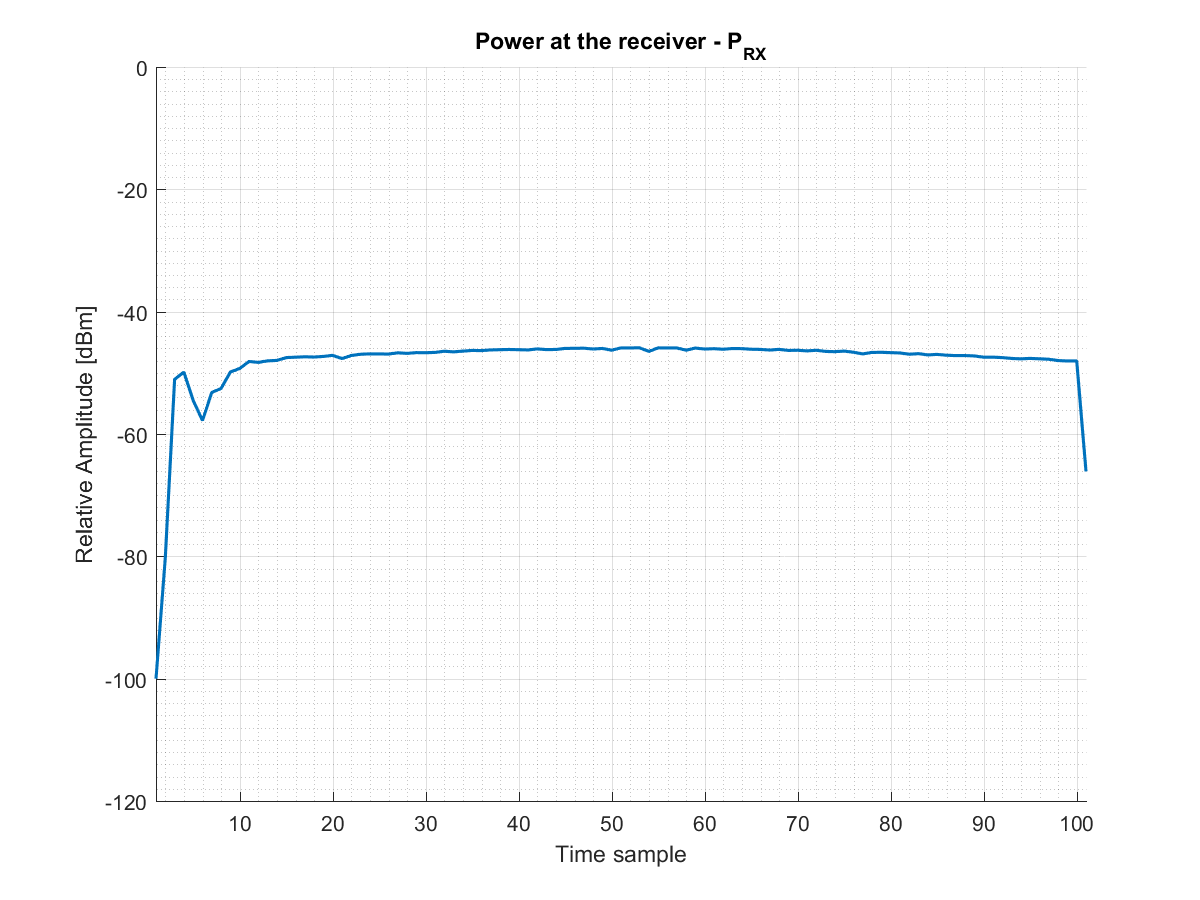
\includegraphics[scale=0.45,angle=-90]{figures/s1_pi_power.png}}
	\hfill
	\\
	\hfill
	\subfigure[PD]{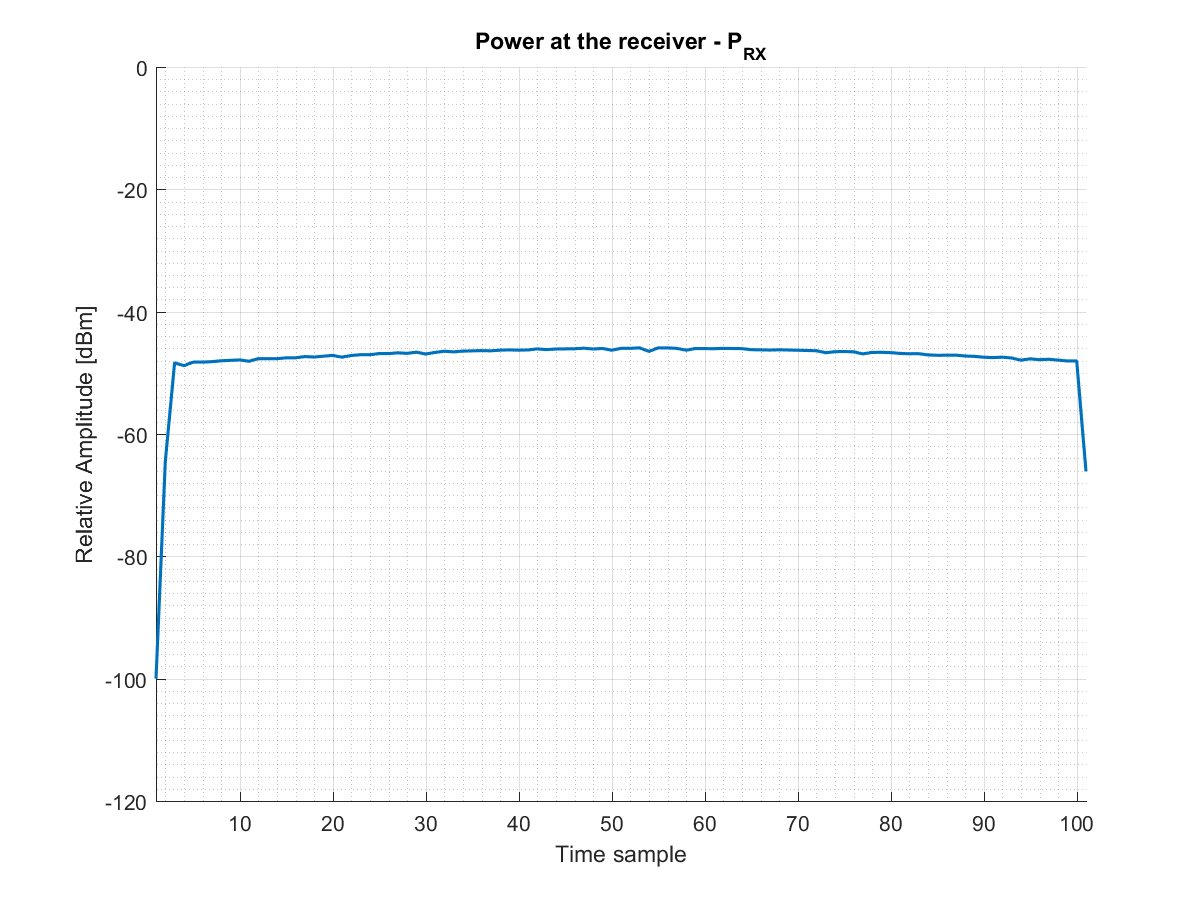
\includegraphics[scale=0.45,angle=-90]{figures/s1_pd_power.png}}
	\hfill
	\subfigure[PID]{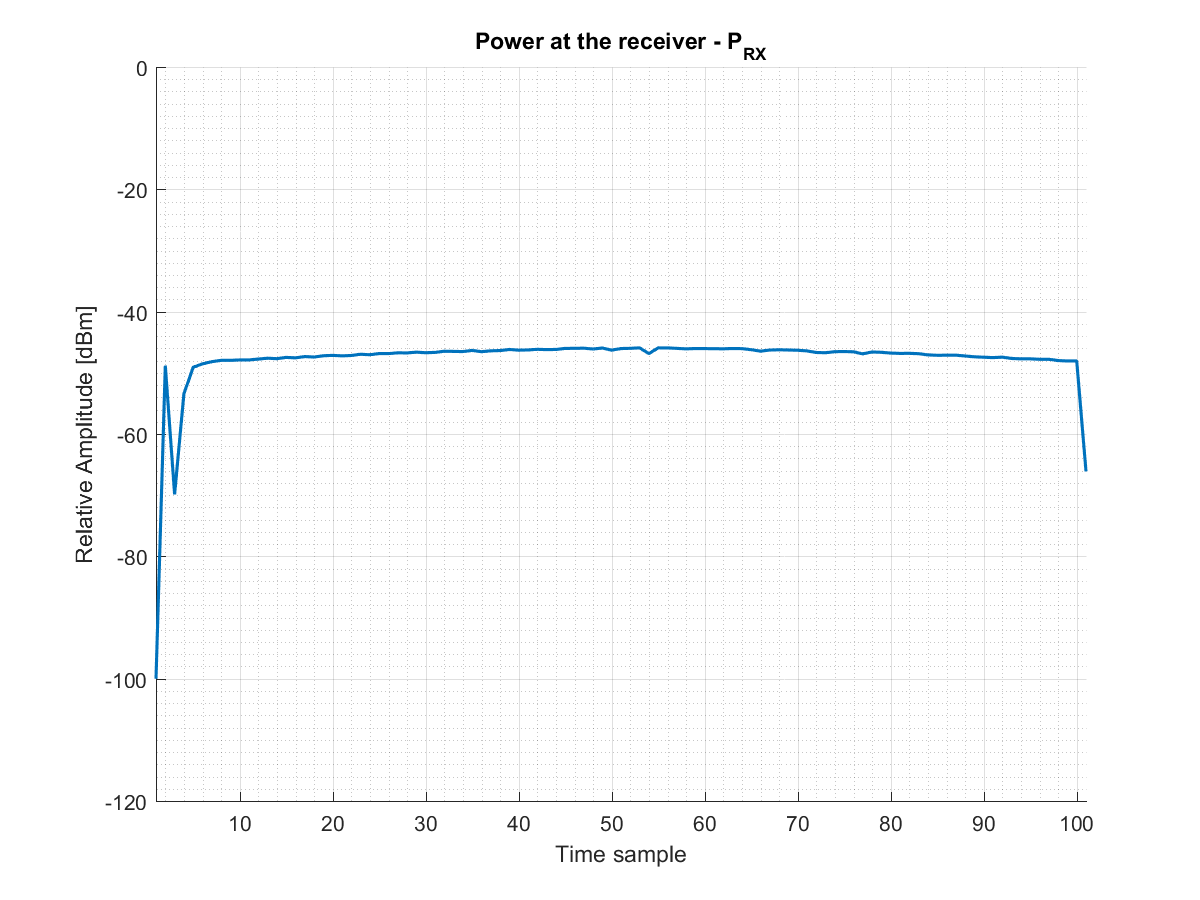
\includegraphics[scale=0.45,angle=-90]{figures/s1_pid_power.png}}
	\hfill
	\caption{Power for each controller}
	\label{fig:s1_power}
\end{figure}
